\documentclass[12pt]{article}
\usepackage{natbib}
\usepackage{hyperref}
\usepackage{graphicx}
\usepackage{subcaption}
\usepackage{amssymb,amsmath,amsthm}
\usepackage{xcolor}
\usepackage{xspace}
\usepackage[nameinlink,capitalize]{cleveref}
\usepackage{cleveref}
\usepackage{geometry}
\usepackage{pdflscape}

\usepackage{xspace}
\newcommand{\Rlogo}{\protect
\includegraphics[height=2ex,keepaspectratio]
{pix/Rlogo.pdf}\xspace}

\newcommand{\comment}{\showcomment}
%% \newcommand{\comment}{\nocomment}

\newcommand{\showcomment}[3]{\textcolor{#1}{\textbf{[#2: }\textsl{#3}\textbf{]}}}
\newcommand{\nocomment}[3]{}

\newcommand{\fady}[1]{\comment{cyan}{Fady}{#1}}
\newcommand{\ali}[1]{\comment{magenta}{Ali}{#1}}
\newcommand{\jd}[1]{\comment{blue}{JD}{#1}}
\newcommand{\djde}[1]{\comment{red}{DJDE}{#1}}
\newcommand{\bmb}[1]{\comment{red}{BMB}{#1}}
\newcommand{\todo}[1]{\comment{red}{TODO}{#1}}

\newcommand{\Rnum}{\mathcal{R}_0}
\theoremstyle{definition} % amsthm only
\newtheorem{prop}{Proposition}
\newtheorem{note}{note}
\newtheorem{theorem}{Theorem}

\bibliographystyle{apalike}

\title{Notes on a Simple Epidemic Model }

\begin{document}
\maketitle

% %%%%%%%
\section{Method}

\subsection{model and parameters}
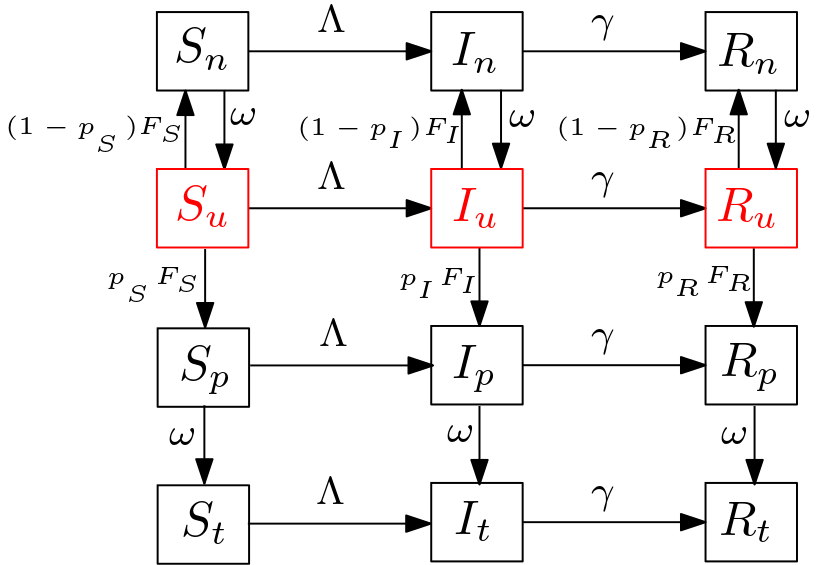
\includegraphics[width=0.5\linewidth]{../pix/sir_comp.png}

The model is
\begin{align}
% \label{model}
 d S_u/dt &= -\Lambda S_u - F_S S_u + \omega S_n, \label{eq1}\\
 d S_n/dt &= -\Lambda S_n + (1-p_S) F_S S_u - \omega S_n, \label{eq2}\\
 d S_p/dt &= -\Lambda S_p + p_S F_S S_u - \omega S_p, \label{eq3}\\
 d S_c/dt &= -\Lambda S_c + \omega S_p, \label{eq4}\\
 d I_u/dt &= \Lambda S_u - F_I I_u + \omega I_n  - \gamma I_u,  \label{eq5}\\
 d I_n/dt &= \Lambda S_n + (1-p_I) F_I I_u - \omega I_n -\gamma I_n, \label{eq6}\\
 d I_p/dt &= \Lambda S_p + p_I F_I I_u - \omega I_p -\gamma I_p, \label{eq7}\\
 d I_c/dt &= \Lambda S_c + \omega I_p - \gamma I_c,  \label{eq8}\\
 d R_u/dt &= \gamma I_u - F_R R_u + \omega R_n, \label{eq9}\\
 d R_n/dt &= \gamma I_n + (1-p_R) F_R R_u - \omega R_n,  \label{eq10}\\
 d R_p/dt &= \gamma I_p + p_R F_R R_u  - \omega R_p,  \label{eq11}\\
 d R_c/dt&= \gamma I_c + \omega R_p,  \label{eq12}\\
 dN/dt &= \omega (S_n + I_n + R_n),   \label{eq13}\\
 dP/dt &= \omega(I_p + R_p) \label{eq14},
\end{align}

\newgeometry{margin=1cm} % modify this if you need even more space
\begin{landscape}
\begin{table}[htp]
\centering
{\tiny %
\begin{tabular}{|c|ccc|} \hline
  Symbol & Description & Unit & Value \\ \hline
  $N_0$     & Total population size & people & $10^6$ \\ \hline
  $\omega$  & Rate of onward flow from the awaiting to reported or untested compartments  & 1/day & - \\ \hline
  $\gamma$ & Recovery rate & 1/day & 1/3 \\ \hline
  $\rho$   & Per capita testing intensity & 1/day & 0.01 \\ \hline
  $\eta_w$  & Relative probability of transmission for isolated awaiting individuals & - & - \\ \hline
  $\eta_c$  & Relative probability of transmission for isolated confirmed individuals & - & -  \\ \hline
  $\Lambda$ & Force of infection & 1/day & - \\ \hline
  $p_S$ & Probability of false positive for susceptible& - & 0 \\ \hline
  $p_I$ & Probability of being infected and tested positive & - & 1 \\ \hline
  $p_R$ & Probability of being recovered and tested positive & - & 0.5 \\ \hline
  $W_S, W_I, W_R$ & Relative testing weight & - &
  \begin{minipage}[t]{0.21\columnwidth}%
 Random testing: $W_S=W_I=W_R=1$, \\Non-random testing: $W_S=0.3, W_I=W_R=1$
\end{minipage} \\ \hline

  \end{tabular}
  }%
\caption{\label{tab:params} The underlying parameters of model, \crefrange{eq1}{eq12}.}
\end{table}
\end{landscape}
\restoregeometry
 
% % %%%%%%%%%%%%%%%%%%%%%%%%%%%%%%%%%%%%%%%%%%%%%%%%%%%%%%%%%%%%%
\section{Results}
% % %%%%%%%%%%%%%%%%%%%%%%%%%
\subsection{On the calculation of $\Rnum$}
\begin{itemize}
\item
{\bf DFE} is given by solving the following system \footnote {Note when $I_u=R_u=0$, $F_S=\frac{\rho N_0}{W_S S_u}$. }
\begin{align*}
S_u+S_n &= N_0 \\
F_S S_u-\omega S_n &= 0
\end{align*}
\item {\bf DFE:}
  \begin{itemize}
    \item[] $S_u = (1-\frac{\rho}{\omega})N_0$,
    \item[] $S_n = \frac{\rho}{\omega} N_0$,
    \item[] $I_j=R_j=0$ \, for all \, $j$.
  \end{itemize}
\item At the DFE, $F_I^* =\frac{\rho }{ (1-\rho/\omega) } W_I/W_S$
also note that $\partial{F_I^*}/\partial{\rho}>0.$
\end{itemize}

\begin{align}
\label{FV}
F =& \beta/N_0 \left[ \begin {array}{cccc}
S_u&\eta_w\,S_u&\eta_w\,S_u&\eta_c\,S_u\\
S_n&\eta_w\,S_n&\eta_w\,S_n&\eta_c\,S_n\\
0&0&0&0\\
0&0&0&0
 \end {array} \right], \\
  V =&
 \left[ \begin {array}{cccc}
F_I+\gamma&-\omega&0&0\\
-(1-p_I)F_I&\omega+\gamma&0&0\\
-p_I F_I&0&\omega+\gamma&0\\
0&0&-\omega&\gamma
\end {array} \right].
\end{align}

Also,
\begin{align}
\label{Vinv}
V^{-1} =&
\left[ \begin {array}{cccc}
\frac {\omega+\gamma}{\hat{F_I}} & \frac {\omega}{\hat{F_I}}&0&0\\
\noalign{\medskip}
\frac{(1-p_I) F_I}{\hat{F_I}}& \frac{F_I+\gamma}{\hat{F_I}}&0&0\\
\noalign{\medskip}
\frac{p_I F_I}{\hat{F_I}}& \frac{\omega p_I F_I}{(\omega+\gamma)\hat{F_I}}& \frac{1}{\omega+\gamma}&0 \\
\noalign{\medskip}
\frac{\omega\,F_I\,p_I}{\gamma \hat{F_I}}&
\frac{\omega^2\,F_I\,p_I}{\gamma(\omega+\gamma) \hat{F_I}}&
\frac{\omega}{\gamma (\omega+\gamma)}&
\frac{1}{\gamma}
\end {array} \right],
\end{align}

where $\hat{F_I}=\gamma(\omega +\gamma)+(\gamma+\omega p_I)F_I$. 


The particular form of $F$ with two rows of zeros at the bottom, simplifies $G$ as
\begin{equation}
G = \left[ \begin {array}{cc}
G_{11}&G_{12}\\
0&0
\end {array} \right], \text{ where } \\
G_{11} =C
\left[\begin {array}{cc}
A\,S_u & B\,S_u\\
A\,S_n & B\,S_n
\end {array}\right].
\end{equation}

The Disease-Free Equilibrium (DFE) for the SIR model, \crefrange{eq1}{eq12}, is given by solving the coupled system including $S_u+S_n=N_0$ and $F_S S_u-\omega S_n=0$. The DFE is

\begin{equation}
\label{dfe}
S_n^*= \frac{\rho}{\omega} N_0, \ S_u^*= N_0-S_n^*, \text{and} I_j=R_j=0 \ \text{for all j}.
\end{equation}

The basic reproduction number, $\Rnum$, was calculated by using the next generation matrix method developed by \cite{van2002reproduction}. $\Rnum$ is

\begin{equation}
\label{R0}
\Rnum= (A \times S_u^* + B \times S_n^*) \times C,
\end{equation}
where
\begin{align*}
A=& \gamma(\omega+\gamma) + (\gamma \eta_w + \omega \eta_c p_I) F_I, \\
B=& \big(\omega+(F_I+\gamma)\eta_w\big) \gamma+\frac{(\eta_w \gamma+ \eta_c\omega) \omega p_I F_I }{\omega+\gamma}, \\
C=& \frac{\beta/\gamma}{N_0 (\gamma(\omega+\gamma)+F_I(\gamma+\omega p_I))}.
\end{align*}

Note that the block matrix $G_{12}$ does not influence $\Rnum$ defined as the spectral radius of $G$. All matters here are the eigenvalues of $G_{11}$, which are 0 and $\Rnum$ \eqref{R0}.
% 
% % %%%%%%%%%%%%%%%%%%%%%%%%%
\subsection{Sensitivity of $\Rnum$ with respect to the underlying parameters}

\begin{note} The tricky one is the $\partial{\Rnum}/\partial{\rho}$; Following JD comment and some analysis, we can prove that analytically.
\end{note}

{\bf Jonathan's comment:} "There should be a logical route to a clear proof about $\rho$. The total
amount of time spent in $I_x$ when starting from a given starting point should not depend on $\rho$ (or anything but $\gamma$). And this should be reflected in the column sums of $V^{-1}$.
Since both of the $\eta$'s are $<1$, all we should then need to prove is that the (nonzero) values on the first row of $V^{-1}$ decrease with $\rho$ to show that the elements of $FV^{-1}$ decrease with $\rho$, which presumably shows that $\Rnum$ decreases as well. This needs to be filled ink but should work."

\begin{note}
\label{note:rankf}
Notice that matrix $F$ is a rank one matrix, thus $FV^{-1}$ is of a rank one. This is why $FV^{-1}$ has only one non-zero eigenvalue. Specifically, $F$ is a rank one means that it can be written as matrix product of a column vector and a row vector as follows
$$
F = \beta/N_0 \left[\begin{array}{c} S_u\\  S_n\\ 0\\ 0 \end {array} \right]
\left[\begin{array}{cccc} 1 \eta_w \eta_w \eta_c \end {array} \right].
$$
\end{note}

\begin{note}
The enteries in the first row of matrix $V^{-1}$ are decreasing wrt $\rho$, which represents that individuals are spending less time in average in untested compartment, $I_u$, as testing intensity increases. On the other hand, the enteries in the other rows of $V^{-1}$ are increasing wrt $\rho$. Thus, the more testing the more waiting or reporting time.5
\end{note}
% 
% \begin{prop}\label{prop1}
% Let $f$ and $g$ be smooth real functions such that (i) $f(x) \leq g(x)$ for all $x \in (x_0,x_0+\epsilon)$ and (ii) $f(x_0)=g(x_0)$, then the definition of the derivative yields
% $$f'(x_0) = \lim_{h\to 0} \frac{f(x_0+h)-f(x_0)}{h} =
% \lim_{h\to 0} \frac{f(x_0+h)-g(x_0)}{h} \leq
% \lim_{h\to 0} \frac{g(x_0+h)-g(x_0)}{h} =
% g'(x_0).
% $$
% \end{prop}
% 
% Based on the note \ref{note:rankf}, Also notice that $FV^{-1}$ is of rank one matrix since it can be written as matrix product of a column vector and a row vector. Thus, the next generation matrix $G=F V^{-1}$ has only one non-zero eigenvalue given by the trace $G$ \footnote {see the argument in  \url{https://www.physicsforums.com/threads/eigenvalues-of-a-rank-1-matrix.682216/}}.
% 
% Thus,
% \begin{equation}
% \mathrm{trace}(G) = \mathrm{trace}(G_{11})
% \leq \frac{\beta}{\gamma} \frac{1}{N_0} (S_u^*+S_n^*) \, \, \,\forall \rho \in (0,\epsilon).
% \end{equation}
% It is easy to show that $\mathrm{trace}(G)= \frac{\beta}{\gamma} \frac{1}{N_0} (S_u^*+S_n^*) =1/\gamma$. Thus, following the Prop.\ref{prop1}, $\partial{\Rnum}{\rho} \leq 0$.



% % %%%%%%%%%%%%%%%%%%%%%%%%%%%%%%%%%%%%%%%%%%%%%%%%%%%%%%%%%%%%%
% \section{Thoughts/Objectives}
% 
% 
% 
% \begin{enumerate}
% \item 
% \begin{itemize}
% \item analysis of the basic SIR model with testing: analytical results as far as possible, supplemented by numerical results as necessary/for illustration. Heuristic explanations/insights of what we learn from this.
% \item Maybe?? order-of-magnitude/back-of-the-envelope calculations of the magnitudes of testing and isolation necessary. (However, the model may be too simplified for even back-of-the-envelope calculations to be meaningful.)
% \item Maybe?? comparison with strength-and-speed framework (since T/T/I is essentially a speed-based intervention)
% \end{itemize}
% 
% \item
% \begin{itemize}
% \item extension to a SEPAIR model (i.e. including latent/exposed, presymptomatic, asymptomatic)
%   (i) analytical results will probably be out of reach
% 	(ii) but it may be possible to extend some of the insights gained in part 1
% 	(iii) in any case, some numerical results (the space of relevant/interesting parameters will be larger: figure out a sensible way to show results from this parameter space. Are there useful dimensionless parameters that could help frame this?)
% \item more detailed quantitative exploration: in particular, *either* Latin hypercube *or* (nearly the same!) a sample over estimated ('prior') distributions of the parameters. Goal: answer the general question "how likely is TTI to be able to control COVID?"
% \end{itemize}
% \end{enumerate}
% 
% 
% % %%%%%%%
% \section{Literature Review}
% 
% \subsection{Explicit models of TTI (trace/test/isolate) based on network or agent-based models}
% 
% \citep{endo2020implication} [Ali: It seems to me that this is just a statistical model to estimate the parent-offspring of an infected index, not sure if it fits into agent-based group!] Used simulation on a branching process model to assess the forward and backward contact tracing efficiency. Assuming a negative-binomial branching process with a mean R, reproduction number, and overdispersion parameter k, the mean total number of generation G3 and averted G3 are estimated. The effectiveness of TTI is defined as the ratio of averted to the mean.
% 
% \citep{jenness2020modeling} developed a network-based transmission model for SARS-CoV-2 on the Diamond Princess outbreak to characterize transmission dynamics and to estimate the epidemiological impact of outbreak control and prevention measures. 
% 
% \citep{elbanna2020entry} [seems similar to MacPan model!]
% 
% \citep{de2020influenza} Was discussed in the Math 747 
% SEIR Asymptomatic and symptomatic $I_1, I_2$. Used linear chain trick 
% Stringency index as a control force lowering $\beta$.
% 
% \citep{rice2020effect} Effect of school closures on mortality. Reproduce Report 9 results by spatial agent based CovidSim. 
% % %%%%%%%
% \subsection{Models of repeated random testing of isolated populations}
% \cite{bergstrom2020frequency}
% (1) Model, assumptions: They developed a function, namely expected exposure $E(C,\tau)$, to approximate trade-offs between the frequency of testing, n, the sensitivity of testing, q, and the delay between
% testing and results, d. This function is explicitly derived and was connected the effective reproduction number $R=R_0 S$, where $S$ is the proportion of population susceptible.
% assumption that transmission rates are a step function: individuals who
% have COVID go from non-infectious to fully infectious instantaneously,
% and remain fully infectious until they are no longer able to transmit disease. Test sensitivity takes the same form over the course of infection.
% More sophisticated models could allow varying infectiousness and varying
% sensitivity over time, as in 
% \citep{larremore2020test}.
% 
% \citep{lopman2020model} Used a Deterministic SEIR model, incorporated TTI, applicable to a university setting. They assumed a fairly high reproductive number that is not reduced through social
% distancing measures. They found that community-introduction of SARS-CoV-2 infection onto campus can be
% relatively controlled with effective testing, isolation, contract tracing and quarantine.
% 
% \citep{tuite2020mathematical} used an age-structured compartmental model of COVID-19 transmission in the population of Ontario, Canada. We compared a base case with limited testing, isolation and quarantine to different scenarios. 
% 
% 
% 
% 
% % %%%%%%%
% \subsection{Other maybe-related works}
% \citep{arino2020simple} developed a SLIAR compartmental model to study the spread of an epidemic, specifically COVID-19, in a population. The model incorporates an Erlang distribution of times of sojourn in incubating, symptomatically and asymptomatically infectious compartments. Basic reproduction number is derived. Also, sensitivity analysis with respect to the underlying parameters for the following two outputs was carried out; (i) the number of observable cases during the course of the epidemic and at the peak, and (ii) the timing of the peak of the outbreak. Sensitivity analysis is performed using the R package multisensi.
% 
% \citep{ruszkiewicz2020diagnosis} novel with-in-a-minute breath testing with 80\% accuracy. 
% %%%%%%%
\bibliography{../SIRlibrary}
\end{document}
